\documentclass{article}
\usepackage{amsmath }
\usepackage{tikz}

\begin{document}

    \begin{center}
        \Huge
        Leminscate of Bernoulli
        \bigskip
        \normalsize
        
        Parametric equation:
        \[x\left(\theta\right)=\dfrac{\cos\theta}{1+\sin^2\theta}~\land~y\left(\theta\right)=\dfrac{\sin\theta\cos\theta}{1+\sin^2\theta}\]
        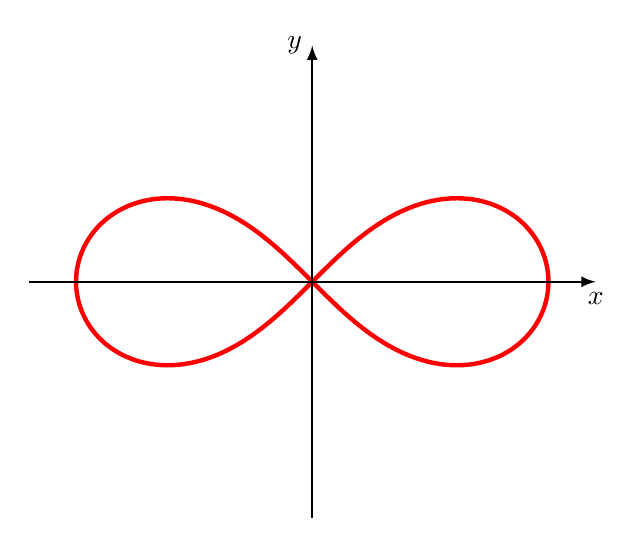
\begin{tikzpicture}[scale=3]
            \draw[color=red, ultra thick, domain=0:2*pi,smooth,variable=\t, samples=300] 
                plot ({cos(\t r)/(1+(sin(\t r))^2)},{0.5*sin(2*\t r)/(1+(sin(\t r))^2)});
    
            \draw[thick, ->, >=latex] (-1.2,0) -- (1.2,0) node[below]{\(x\)};
            \draw[thick, ->, >=latex] (0,-1) -- (0,1) node[left]{\(y\)};        
    
        \end{tikzpicture}    
    \end{center}

\end{document}
